\documentclass[a4paper,11pt]{jsarticle}


% 数式
\usepackage{amsmath,amsfonts,amssymb}
\usepackage{bm}
% 画像
\usepackage[dvipdfmx]{graphicx}
\usepackage{siunitx}
\usepackage{wrapfig}
\usepackage{cases}
\usepackage{dcolumn}
\makeatletter
\newcommand{\figcaption}[1]{\def\@captype{figure}\caption{#1}}
\newcommand{\tblcaption}[1]{\def\@captype{table}\caption{#1}}
\makeatother

\usepackage{listings,jvlisting}
\lstset{
basicstyle={\ttfamily},
identifierstyle={\small},
commentstyle={\smallitshape},
keywordstyle={\small\bfseries},
ndkeywordstyle={\small},
stringstyle={\small\ttfamily},
frame={tb},
breaklines=true,
columns=[l]{fullflexible},
numbers=left,
xrightmargin=0zw,
xleftmargin=3zw,
numberstyle={\scriptsize},
stepnumber=1,
numbersep=1zw,
lineskip=-0.5ex
}

\begin{document}

\title{閉ループに関して}
\author{平林広}
\date{\today}
\maketitle

閉ループの運動方程式が立てられなかった。
「210529\_壁に立てかけた棒」において、
古めの考えが述べられている。
しかしそれは嘘であった。

\begin{figure}[h]
  \centering
  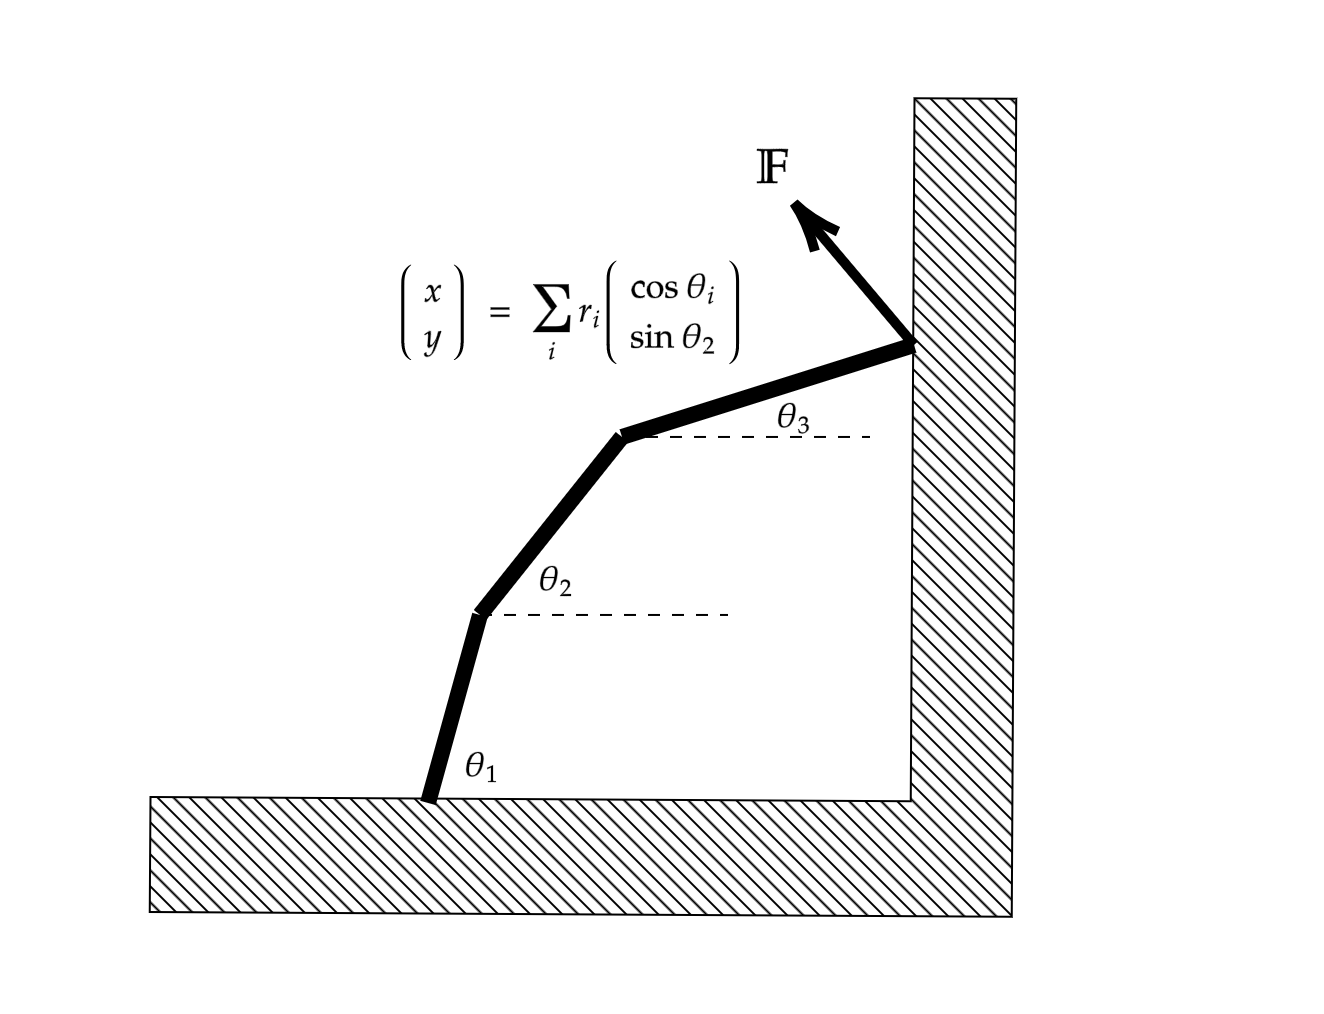
\includegraphics[width = 1\textwidth]{ex_Triple_Pendulum.png}
  \caption{3重振り子の例}
  \label{fig:ex_Triple_Pendulum}
\end{figure}

このような状況を考える。
ラグランジアンはこんな風になる。
\begin{align*}
  \Theta_1 + \mathbb{F}_x \frac{\partial x}{\partial \theta_1} + \mathbb{F}_x \frac{\partial x}{\partial \theta_1}
  & = \frac{d}{dt}\frac{\partial L}{\partial \dot{\theta}_1} - \frac{\partial L}{\partial \theta_1}
  \\ \Theta_2 + \mathbb{F}_x \frac{\partial x}{\partial \theta_2} + \mathbb{F}_x \frac{\partial x}{\partial \theta_2}
  & = \frac{d}{dt}\frac{\partial L}{\partial \dot{\theta}_2} - \frac{\partial L}{\partial \theta_2}
  \\ & \vdots
  \\ \Theta_i + \mathbb{F}_x \frac{\partial x}{\partial \theta_i} + \mathbb{F}_x \frac{\partial x}{\partial \theta_i}
  & = \frac{d}{dt}\frac{\partial L}{\partial \dot{\theta}_i} - \frac{\partial L}{\partial \theta_i}
  \\ & \vdots
\end{align*}
これに加えて拘束条件である、
\begin{align*}
  \dot{x} &= 0 \\
  \dot{y} &= 0
\end{align*}
が存在する。
この2条件は$\dot{\theta_i}$に関して一時線形であるから、容易に解ける。

例えば2次元の場合は$\mathbb{F}$が2要素を持っているので、
$\mathbb{F}$に関する式が2つ要る。
だから2重振り子以上で$\mathbb{F}$が定まる。
2重振り子だと拘束条件から$\dot{\theta}_1, \dot{\theta}_2$が定まるから、
形が完全に定まる。
3重振り子以上だと冗長性が出てくる。

3次元だと1セグメントごとに2自由度存在する。
つまり2重振り子で4自由度。
$\mathbb{F}$が3要素だから
実は3次元で形が定まるパターンは存在しない。

実際に運動方程式を導くときは、
\begin{align*}
  \dot{x} &= 0 \\
  \dot{y} &= 0 \\
  \Theta_1 + \mathbb{F}_x \frac{\partial x}{\partial \theta_1} + \mathbb{F}_x \frac{\partial x}{\partial \theta_1}
  & = \frac{d}{dt}\frac{\partial L}{\partial \dot{\theta}_1} - \frac{\partial L}{\partial \theta_1}
  \\ \Theta_2 + \mathbb{F}_x \frac{\partial x}{\partial \theta_2} + \mathbb{F}_x \frac{\partial x}{\partial \theta_2}
  & = \frac{d}{dt}\frac{\partial L}{\partial \dot{\theta}_2} - \frac{\partial L}{\partial \theta_2}
  \\ & \vdots
  \\ \Theta_i + \mathbb{F}_x \frac{\partial x}{\partial \theta_i} + \mathbb{F}_x \frac{\partial x}{\partial \theta_i}
  & = \frac{d}{dt}\frac{\partial L}{\partial \dot{\theta}_i} - \frac{\partial L}{\partial \theta_i}
  \\ & \vdots
\end{align*}
で解くパターンと
\begin{align*}
  \ddot{x} &= 0 \\
  \ddot{y} &= 0 \\
  \Theta_1 + \mathbb{F}_x \frac{\partial x}{\partial \theta_1} + \mathbb{F}_x \frac{\partial x}{\partial \theta_1}
  & = \frac{d}{dt}\frac{\partial L}{\partial \dot{\theta}_1} - \frac{\partial L}{\partial \theta_1}
  \\ \Theta_2 + \mathbb{F}_x \frac{\partial x}{\partial \theta_2} + \mathbb{F}_x \frac{\partial x}{\partial \theta_2}
  & = \frac{d}{dt}\frac{\partial L}{\partial \dot{\theta}_2} - \frac{\partial L}{\partial \theta_2}
  \\ & \vdots
  \\ \Theta_i + \mathbb{F}_x \frac{\partial x}{\partial \theta_i} + \mathbb{F}_x \frac{\partial x}{\partial \theta_i}
  & = \frac{d}{dt}\frac{\partial L}{\partial \dot{\theta}_i} - \frac{\partial L}{\partial \theta_i}
  \\ & \vdots
\end{align*}
で解くパターンが存在する。
どちらで解いてももちろん同じ解になるが、
matlabのode45で数値積分すると、
前者の速度から出すパターンは値が発散する。
後者の加速度から出すパターンは固定点がだんだんずれる


\section{編集日付}
\begin{itemize}
  \item 2021/05/31
\end{itemize}





\end{document}